% =====================================================================
% main.tex -- IEEE conference paper
% Build: pdflatex main -> bibtex main -> pdflatex main (x2)
% Bibliography: refs.bib | Figures: figures/ | Tables III and IV: tables/ (python make_tables.py)
% =====================================================================

\documentclass[conference]{IEEEtran}
\IEEEoverridecommandlockouts

% ---------------------------------------------------------------------
% Packages
% ---------------------------------------------------------------------
\usepackage{cite}                    % sorted/compressed citations [1]-[3]
\usepackage{amsmath,amssymb,amsfonts}% math
\usepackage{graphicx}                % \includegraphics
\usepackage{booktabs}                % \toprule, \midrule, \bottomrule
\usepackage{multirow}                % multi-row table cells
\usepackage{xcolor}                  % colors (used by \todo and TikZ)
\usepackage{url}                     % \url{}
\usepackage{tikz}                    % framework diagram (Fig. 1)
\usetikzlibrary{positioning,arrows.meta,fit,calc}

% ---------------------------------------------------------------------
% Custom commands
% ---------------------------------------------------------------------
% Red notes for things still to check. Remove all of them before submission.
\newcommand{\todo}[1]{\textcolor{red}{[TODO: #1]}}
% Table rows written by make_tables.py; the primitive \input also works inside a tabular
\makeatletter\newcommand{\inputtable}[1]{\@@input #1 }\makeatother

\begin{document}

% =====================================================================
% Title and authors
% =====================================================================
\title{Classification of Marine Incident Reports Using Transformer-Based Language Models}

% TODO: confirm the author list and order with the supervisor.
\author{
\IEEEauthorblockN{Mohammad Mahdi Arab}
\IEEEauthorblockA{\textit{Department of Computer Engineering}\\
\textit{Shahrood University of Technology}\\
Shahrood, Iran\\
math.mohammad.arab@shahroodut.ac.ir}
\and
\IEEEauthorblockN{Hoda Mashayekhi}
\IEEEauthorblockA{\textit{Department of Computer Engineering}\\
\textit{Shahrood University of Technology}\\
Shahrood, Iran\\
hmashayekhi@shahroodut.ac.ir}
\and
\IEEEauthorblockN{Maryam Khodabakhsh}
\IEEEauthorblockA{\textit{Department of Computer Engineering}\\
\textit{Shahrood University of Technology}\\
Shahrood, Iran\\
m\_khodabakhsh@shahroodut.ac.ir}
}

\maketitle

% =====================================================================
% Abstract and keywords
% =====================================================================
\begin{abstract}
In response to the growing volume of marine accident and incident reports and the rarity of the most safety-critical incident types, this study develops a framework for the automatic classification of marine incident reports that integrates a pre-trained Bidirectional Encoder Representations from Transformers (BERT) model with a Bidirectional Long Short-Term Memory network (BiLSTM) and an attention layer. To address class imbalance, the framework is combined with re-weighted loss functions, oversampling and data augmentation with a large language model (LLM). Using 5,762 public incident reports of the UK Marine Accident Investigation Branch (MAIB) in nine classes, all models are trained under identical settings with two random seeds and compared with a TF-IDF + support vector machine (SVM) baseline. Systematic performance comparisons show that the best configuration, BERT + BiLSTM + attention trained with inverse-frequency weighted cross-entropy on LLM-augmented data, attains a macro-F1 of 0.915 and an accuracy of 93.5\%, against 0.885 and 91.4\% for the baseline. The weighted loss provides most of this gain, whereas the BiLSTM and attention layers, as well as a larger BiLSTM, do not improve on plain BERT beyond seed-to-seed variation, and pairwise significance tests find no significant difference among the BERT-based configurations on the 865-report test set. Attention and error analyses reveal a hidden group of reports on non-compliant pilot ladders and show that most remaining errors occur between cause and consequence classes. The framework provides maritime authorities with an automatic and interpretable tool for coding incident reports, and the results indicate that better annotation schemes, rather than more complex architectures, are the main lever for further improvement.
\end{abstract}

\begin{IEEEkeywords}
marine incident reports; text classification; BERT; BiLSTM; attention; class imbalance; data augmentation; large language model
\end{IEEEkeywords}

% =====================================================================
% 1. Introduction
%    Context, challenges (with references), the reference work and its open issues, this study, organization
% =====================================================================
\section{Introduction}

Shipping remains one of the most hazardous transport sectors, and marine accidents such as collisions, groundings, fires, flooding and capsizing cause loss of life, damage to vessels and cargo, and pollution \cite{zhao2025causation}. National investigation bodies, such as the UK Marine Accident Investigation Branch (MAIB), record every reported accident and incident as a short narrative together with its type. These narratives are a key source for safety learning: once they are coded consistently, they reveal which incident types are frequent, which are increasing, and which call for new regulations \cite{black2026domain}. The coding, however, is still done manually by experts, which is slow and depends on the coder. Automatic classification of the narratives can make this process faster and more consistent.

Automatic classification of incident reports faces three challenges. First, the classes are highly imbalanced: in the MAIB data, accidents to persons outnumber capsizing incidents by a factor of about 17 \cite{munaev2025maib}, and the most safety-critical types, such as fire, flooding and capsizing, are among the rarest. A model trained to maximize overall accuracy can largely ignore them, a well-known problem of learning from long-tailed data \cite{lin2017focal,cui2019classbalanced}. Second, each report carries a single label although many incidents are a chain of events, for example an engine failure that leads to a grounding; the label then names only one link of the chain \cite{zhao2025causation}. Third, the reports use a specialized maritime vocabulary that general-purpose language models rarely see during pre-training \cite{black2026domain}.

Pre-trained Transformer encoders such as BERT \cite{devlin2019bert} have recently been applied to maritime accident texts \cite{zhao2025causation,black2026domain,yu2026semantic,wang2026fire}. In particular, Zhao et al.\ \cite{zhao2025causation} combined BERT with a BiLSTM to classify accident causes and reported that this architecture outperforms plain BERT, reaching an accuracy of 89.8\%. However, three issues of that study remain open. The compared models were trained with different dropout, regularization, gradient-clipping and activation settings, so the gain may come from the settings rather than from the architecture; no repeated runs were reported, so the size of random variation between runs is unknown; and the main metric was accuracy, which hides the performance on rare classes. Moreover, the data are not public, so the results cannot be reproduced.

This study addresses these issues on a public dataset. We develop a framework that adds an attention layer over the BiLSTM states of a BERT encoder, compare it with plain BERT and with the BERT + BiLSTM model of \cite{zhao2025causation} under one training recipe and two random seeds, and evaluate three families of methods against class imbalance: re-weighted loss functions, oversampling and paraphrasing of rare-class reports with an LLM. All models are assessed with macro-F1, the recall of the safety-critical classes and pairwise significance tests. The main contributions are as follows:
\begin{itemize}
  \item a controlled evaluation of BERT, BERT + BiLSTM and BERT + BiLSTM + attention with a shared encoder, an identical training recipe, repeated runs, a classical baseline and significance tests;
  \item a systematic comparison of three loss functions, oversampling and LLM-based data augmentation with a label-consistency filter, with a focus on safety-critical classes;
  \item an error and attention analysis showing that the remaining errors are concentrated between related classes, mostly cause and consequence pairs, and that attention can reveal hidden subgroups within a class;
  \item a fully reproducible pipeline on public data.
\end{itemize}

This paper is organized as follows: Section~\ref{sec:lit} reviews related work, Section~\ref{sec:method} introduces the framework, the models and the imbalance treatments, Section~\ref{sec:eval} describes the evaluation and discusses the results, and Section~\ref{sec:conc} concludes.

% =====================================================================
% 2. Related Work
% =====================================================================
\section{Related Work}\label{sec:lit}

\subsection{Text Analysis of Maritime Accident Reports}

Accident analysis has long been central to maritime safety research. Classical studies coded accident reports manually, for example into human, vessel, environmental and management factors, and analyzed the codes with statistical or causal models \cite{zhao2025causation}. As the number of reports grew, natural language processing (NLP) began to replace part of this manual work. Recent studies rely on pre-trained Transformer encoders. Zhao et al.\ \cite{zhao2025causation} classified the causes of marine traffic accidents on China's coasts into 32 categories with BERT + BiLSTM and reported an accuracy of 89.8\%, followed by Apriori association-rule mining of the predicted causes. Black et al.\ \cite{black2026domain} built a domain-adapted BERT model to classify human factors in maritime accident reports according to the SHIELD taxonomy and showed that domain adaptation helps on maritime vocabulary. Yu et al.\ \cite{yu2026semantic} constructed a knowledge graph of ship collision reports, extracting entities with BERT--BiLSTM--CRF variants and classifying accident severity. Wang et al.\ \cite{wang2026fire} combined ontology-based information extraction, using XLM-RoBERTa with a BiLSTM--CRF tagger, with a dynamic Bayesian network to model the evolution of ship fire and explosion accidents. A BiLSTM on top of a Transformer encoder is therefore a recurring design in this domain, which makes it important to test whether it is actually needed. In parallel, large language models have entered the maritime domain, for example as a maritime question-answering model \cite{nguyen2025llamarine} and for trajectory prediction and collision-risk assessment \cite{park2025aisllm}, but, to our knowledge, their use for generating training data for rare accident classes has not been examined.

\subsection{Class Imbalance and Data Augmentation}

Methods for imbalanced classification act either on the loss or on the data. Loss-level methods give more weight to rare classes: inverse-frequency weighting scales the loss of each class by the inverse of its size, the focal loss \cite{lin2017focal} down-weights examples that the model already classifies with confidence, and the class-balanced loss \cite{cui2019classbalanced} weights each class by the inverse of its effective number of samples. Data-level methods change the training set: random oversampling repeats reports of the small classes, and synthetic sampling such as SMOTE \cite{chawla2002smote} interpolates between examples, which is not directly suited to text. For text, data augmentation ranges from simple edits such as synonym replacement \cite{wei2019eda} and back-translation \cite{sennrich2016improving} to generation with language models whose outputs are filtered by a classifier \cite{anabytavor2020lambada}. For pre-trained Transformers, task-agnostic augmentation has been reported to give only small gains \cite{longpre2020effective}.

This study differs from previous work in three respects. First, it compares the architectures of \cite{zhao2025causation} under one training recipe and with repeated runs, so that the effect of each layer can be isolated. Second, it compares loss-level and data-level imbalance treatments, including LLM-based augmentation, on the same data and with the same protocol, instead of studying them in isolation. Third, it evaluates the models with macro-F1, the recall of the safety-critical classes and significance tests, rather than accuracy alone.

% =====================================================================
% 3. Methodology
% =====================================================================
\section{Methodology}\label{sec:method}

% ---------------------------------------------------------------------
\subsection{Framework}

Fig.~\ref{fig:framework} shows the proposed framework. A report is split into word-pieces and encoded by BERT, a BiLSTM reads the resulting token vectors in both directions, an attention layer pools the BiLSTM states into one vector, and a linear layer with softmax predicts one of the nine incident types. During training, the predicted probabilities and the true label enter a loss function, and its gradient updates all layers, including BERT. The imbalance treatments act at two points of this pipeline: the loss function (Section~\ref{sec:loss}) and the training data (Sections~\ref{sec:oversampling} and \ref{sec:augmentation}).

% --- Fig. 1: framework diagram (drawn with TikZ) ---------------------
\begin{figure}[t]
\centering
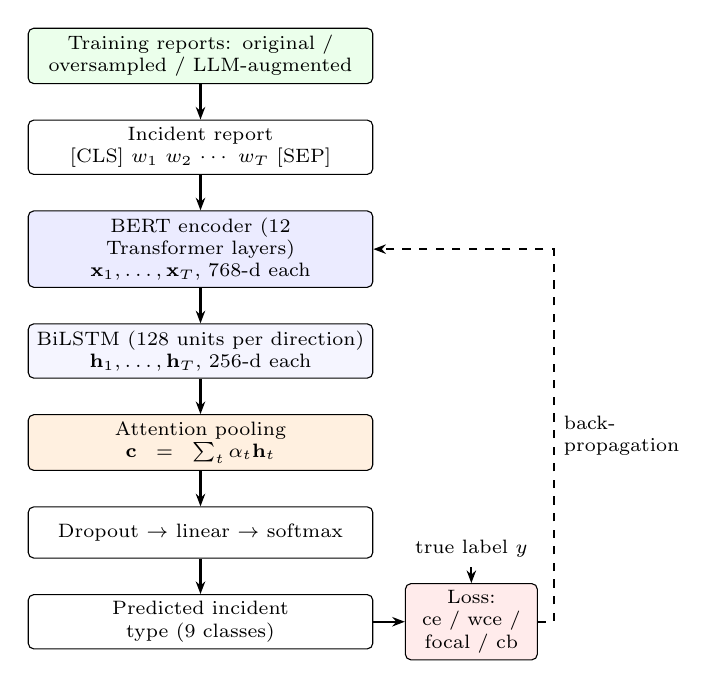
\begin{tikzpicture}[
  node distance=4.5mm,
  box/.style={draw, rounded corners=2pt, align=center, font=\scriptsize,
              minimum height=6.5mm, inner sep=2.5pt, text width=42mm},
  side/.style={draw, rounded corners=2pt, align=center, font=\scriptsize,
               minimum height=6.5mm, inner sep=2.5pt, text width=15mm},
  arr/.style={-{Stealth[length=1.6mm]}, thick}]

  % Main pipeline, fed by the training data
  \node[box, fill=green!8] (data) {Training reports: original / oversampled / LLM-augmented};
  \node[box, below=of data] (in) {Incident report\\{[CLS]} $w_1$ $w_2$ $\cdots$ $w_T$ {[SEP]}};
  \node[box, below=of in, fill=blue!8] (bert)
    {BERT encoder (12 Transformer layers)\\$\mathbf{x}_1, \dots, \mathbf{x}_T$, 768-d each};
  \node[box, below=of bert, fill=blue!4] (lstm)
    {BiLSTM (128 units per direction)\\$\mathbf{h}_1, \dots, \mathbf{h}_T$, 256-d each};
  \node[box, below=of lstm, fill=orange!12] (att)
    {Attention pooling\\$\mathbf{c} = \sum_t \alpha_t \mathbf{h}_t$};
  \node[box, below=of att] (clf)
    {Dropout $\rightarrow$ linear $\rightarrow$ softmax};
  \node[box, below=of clf] (out) {Predicted incident type (9 classes)};

  % Loss (right)
  \node[side, right=4mm of out, fill=red!8] (loss)
    {Loss:\\ce / wce / focal / cb};
  \node[font=\scriptsize, above=2mm of loss] (label) {true label $y$};

  % Arrows
  \draw[arr] (data) -- (in);
  \draw[arr] (in) -- (bert);
  \draw[arr] (bert) -- (lstm);
  \draw[arr] (lstm) -- (att);
  \draw[arr] (att) -- (clf);
  \draw[arr] (clf) -- (out);
  \draw[arr] (out) -- (loss);
  \draw[arr] (label) -- (loss);
  \draw[arr, dashed] (loss.east) -- ++(2mm,0) |- node[pos=0.25, right, font=\scriptsize, align=left]
    {back-\\propagation} (bert.east);
\end{tikzpicture}
\caption{The proposed framework. A report is encoded by BERT, read by a BiLSTM and pooled by attention; a linear layer predicts the incident type. The loss compares the prediction with the true label and its gradient fine-tunes all layers. Imbalance is treated through the loss function or through the training data.}
\label{fig:framework}
\end{figure}

% ---------------------------------------------------------------------
\subsection{BERT Encoder}

We use \texttt{bert-base-uncased} \cite{devlin2019bert}, a 12-layer Transformer \cite{vaswani2017attention} pre-trained on general English text. A report is split into word-pieces $w_1, \dots, w_T$, and the special tokens \texttt{[CLS]} and \texttt{[SEP]} are added at the start and the end. BERT turns each token into a 768-dimensional vector,
\begin{equation}
  [\mathbf{x}_{\mathrm{CLS}}, \mathbf{x}_1, \dots, \mathbf{x}_T] = \mathrm{BERT}(w_1, \dots, w_T),
\end{equation}
where $\mathbf{x}_{\mathrm{CLS}}$ is the vector of the \texttt{[CLS]} token.
Each vector $\mathbf{x}_t$ depends on the whole report through self-attention, so the same word receives different vectors in different contexts. All BERT weights are fine-tuned on our task.

% ---------------------------------------------------------------------
\subsection{BiLSTM Layer}

Following \cite{zhao2025causation}, the token vectors are fed into a BiLSTM \cite{hochreiter1997lstm,schuster1997bidirectional} with 128 units per direction:
\begin{equation}
\begin{aligned}
  \overrightarrow{\mathbf{h}}_t &= \mathrm{LSTM}_{f}(\mathbf{x}_t, \overrightarrow{\mathbf{h}}_{t-1}), \quad
  \overleftarrow{\mathbf{h}}_t = \mathrm{LSTM}_{b}(\mathbf{x}_t, \overleftarrow{\mathbf{h}}_{t+1}), \\
  \mathbf{h}_t &= [\overrightarrow{\mathbf{h}}_t ; \overleftarrow{\mathbf{h}}_t].
\end{aligned}
\end{equation}
The forward LSTM reads the report from left to right and the backward LSTM from right to left; each keeps a memory of the tokens it has read so far through its input, forget and output gates. Concatenating the two states gives a 256-dimensional vector $\mathbf{h}_t$ that summarizes the context on both sides of token $t$. The BERT + BiLSTM model of \cite{zhao2025causation} classifies the report from the two final states, $[\overrightarrow{\mathbf{h}}_T ; \overleftarrow{\mathbf{h}}_1]$. Padding tokens are skipped, so each direction stops at the true end of the report.

% ---------------------------------------------------------------------
\subsection{Attention Layer}

The final states of the BiLSTM must carry the whole report, and the words that decide the incident type, such as \emph{grounded} or \emph{smoke}, often appear in the middle of the narrative. Instead of keeping only the final states, the proposed model pools all BiLSTM states with additive attention \cite{bahdanau2015neural,zhou2016attention}:
\begin{equation}
\begin{aligned}
  e_t &= \mathbf{v}^\top \tanh(\mathbf{W}\mathbf{h}_t + \mathbf{b}), \quad
  \alpha_t = \frac{\exp(e_t)}{\sum_{k}\exp(e_k)}, \\
  \mathbf{c} &= \textstyle\sum_t \alpha_t \mathbf{h}_t.
\end{aligned}
\end{equation}
The score $e_t$ measures how useful token $t$ is for the classification; $\mathbf{W}$, $\mathbf{b}$ and $\mathbf{v}$ are trainable, and the scoring layer has 128 units. The softmax turns the scores into weights $\alpha_t$ that are positive and sum to one over the real tokens of the report; padding tokens receive zero weight. The report vector $\mathbf{c}$ is the weighted average of all states, so informative words contribute more regardless of their position. The weights $\alpha_t$ are stored and later used to inspect which words the model relied on.

% ---------------------------------------------------------------------
\subsection{Classification Layer and Loss Functions}\label{sec:loss}

The pooled vector passes through dropout with rate 0.1 and a linear layer with softmax,
\begin{equation}
  \hat{\mathbf{p}} = \mathrm{softmax}(\mathbf{W}_o\, \mathrm{dropout}(\mathbf{c}) + \mathbf{b}_o),
\end{equation}
where $\hat{\mathbf{p}}$ holds the predicted probability of each of the $K = 9$ classes and the class with the highest probability is the prediction. For a batch of $B$ reports, let $p_i$ be the predicted probability of the true class $y_i$ of report $i$, $N$ the number of training reports and $n_c$ the number of training reports of class $c$. We compare four loss functions.

\textbf{Cross-entropy (ce)} is the standard loss and treats all reports equally:
\begin{equation}
  L_{\mathrm{ce}} = -\frac{1}{B}\sum_{i=1}^{B} \log p_i .
\end{equation}
Since most reports belong to a few large classes, the loss is dominated by them.

\textbf{Weighted cross-entropy (wce)} multiplies the loss of each report by the weight of its class,
\begin{equation}
  L_{\mathrm{wce}} = -\frac{\sum_i w_{y_i} \log p_i}{\sum_i w_{y_i}}, \qquad w_c = \frac{N}{K\, n_c}.
\end{equation}
The weight is the inverse of the class frequency, scaled so that a class of average size has weight one. An error on the rarest class (Capsizing) therefore costs about 17 times more than an error on the largest class, and every class contributes about equally to the total loss.

\textbf{Focal loss} \cite{lin2017focal} reduces the loss of reports that are already classified with confidence:
\begin{equation}
  L_{\mathrm{focal}} = -\frac{1}{B}\sum_{i=1}^{B} (1-p_i)^{\gamma} \log p_i, \qquad \gamma = 2.
\end{equation}
For $p_i$ close to one, the factor $(1-p_i)^{\gamma}$ is close to zero, so training concentrates on hard reports, which are often those of rare classes. The focal loss does not use class sizes.

\textbf{Class-balanced loss (cb)} \cite{cui2019classbalanced} replaces the class size by the effective number of samples, $(1-\beta^{n_c})/(1-\beta)$, which grows more slowly than $n_c$ because many reports of a large class are similar:
\begin{equation}
  w_c = K\,\frac{(1-\beta)/(1-\beta^{n_c})}{\sum_{k} (1-\beta)/(1-\beta^{n_k})}, \qquad \beta = 0.999,
\end{equation}
and the weights are used as in wce. The result is a milder version of inverse-frequency weighting. All class weights are computed on the training set only.

% ---------------------------------------------------------------------
\subsection{Oversampling}\label{sec:oversampling}

Instead of changing the loss, oversampling changes how often each report is seen. For BERT, each training report $i$ is drawn with replacement with probability
\begin{equation}
  P(i) = \frac{1/n_{y_i}}{\sum_{j=1}^{N} 1/n_{y_j}} = \frac{1}{K\, n_{y_i}},
\end{equation}
so every class is drawn with the same probability $1/K$, while the epoch length stays $N$ reports. In expectation, a report of class $c$ is then seen $N/(K n_c) = w_c$ times per epoch, the same factor as the wce weight, but with random variation, and many reports of the large classes are not seen at all in a given epoch. Oversampling is combined with ce rather than wce, since the combination would compensate the imbalance twice. For the SVM baseline, reports of the smaller classes are duplicated at random until every class matches the largest one.

% ---------------------------------------------------------------------
\subsection{LLM-Based Data Augmentation}\label{sec:augmentation}

Oversampling repeats existing reports and adds no new wording. We therefore paraphrase real training reports of the rare classes with \texttt{Qwen2.5-1.5B-Instruct} \cite{qwen2024qwen25}, run locally, until each class with fewer than 400 training reports reaches 400. The prompt asks the model to rewrite the report with different words and sentence structure, to keep every fact (vessel type, event, cause, injuries and damage), and not to name the incident category, so that the classifier cannot learn a shortcut. A rewrite is discarded if its length ratio to the original lies outside $[0.5, 2]$, if its word overlap with the original (Jaccard index) lies outside $[0.15, 0.8]$, i.e., it is a near copy or a different story, or if it duplicates another rewrite. Following LAMBADA \cite{anabytavor2020lambada}, a TF-IDF + SVM trained only on the real training reports must also assign each rewrite to the class of its source report; rejected rewrites are replaced by new ones. The validation and test sets are never shown to the LLM.

% =====================================================================
% 4. Evaluation
%    Data, settings and parameters, baselines, metrics, results, discussion
% =====================================================================
\section{Evaluation}\label{sec:eval}

% ---------------------------------------------------------------------
\subsection{Data}

We use the public MAIB incident dataset \cite{munaev2025maib}, which contains 5,768 short narratives labelled by MAIB with the main event type. We keep the original labels. After removing one exact duplicate and two classes with fewer than 20 reports (Hull Failure, 3; Non-accidental Event, 2), 5,762 reports in nine classes remain. Reports have a median length of 59 words (mean 66.8). The ratio between the largest and the smallest class is 16.8. We split the data once into training (70\%), validation (15\%) and test (15\%) sets, stratified by class and with a fixed seed, and use the same split for all models (Table~\ref{tab:data}). Fire, Capsizing and Flooding are treated as safety-critical classes. Of the 1,493 rewrites generated by the LLM for the rare classes that passed the length, overlap and duplicate checks, 1,068 (71.5\%) also passed the label check, which enlarged the training set from 4,033 to 5,101 reports; the validation and test sets contain real reports only.

% --- Table I: class distribution and split sizes ---------------------
\begin{table}[t]
\caption{Class distribution of the MAIB dataset after cleaning. * marks safety-critical classes.}
\label{tab:data}
\centering
\footnotesize
\begin{tabular}{lrrrr}
\toprule
Class & Total & Train & Val & Test \\
\midrule
Accident to person(s) & 1,662 & 1,163 & 249 & 250 \\
Damage / Loss of Equipment & 1,374 & 962 & 206 & 206 \\
Loss of Control & 823 & 576 & 123 & 124 \\
Grounding / Stranding & 561 & 393 & 84 & 84 \\
Contact & 406 & 284 & 61 & 61 \\
Collision & 326 & 228 & 49 & 49 \\
Fire / Explosion* & 324 & 227 & 49 & 48 \\
Flooding / Foundering* & 187 & 131 & 28 & 28 \\
Capsizing / Listing* & 99 & 69 & 15 & 15 \\
\midrule
Total & 5,762 & 4,033 & 864 & 865 \\
\bottomrule
\end{tabular}
\end{table}

% ---------------------------------------------------------------------
\subsection{Experimental Settings and Parameters}

All BERT-based models use the same recipe (Table~\ref{tab:settings}), so that differences in results can only come from the head, the loss or the data. For each run, the epoch with the highest validation macro-F1 is selected, and the test set is used only once, at the end of the run. Each configuration is trained with two seeds, and we report the mean and sample standard deviation. The recipe deliberately differs from the per-model settings of \cite{zhao2025causation}, which use a learning rate of $10^{-6}$ for all layers, including the newly initialized ones, and would therefore need far more epochs than our budget allows; using one recipe for all models is what allows their effects to be compared. We also train the attention model with a larger BiLSTM, with 384 units per direction (a 768-dimensional output, the size of BERT's vectors), with two layers, or with both. One run took about 75 minutes on a laptop GPU (NVIDIA GTX 1650 Ti, 4 GB), and about 92 minutes with the augmented training set.

% --- Table II: shared training recipe --------------------------------
\begin{table}[t]
\caption{Training settings shared by all BERT-based models.}
\label{tab:settings}
\centering
\footnotesize
\begin{tabular}{ll}
\toprule
Setting & Value \\
\midrule
Encoder & \texttt{bert-base-uncased} \\
Max.\ length & 192 word-pieces (about 2\% truncated) \\
BiLSTM & 128 units per direction, 1 layer \\
Attention & 128-unit scoring layer \\
Dropout & 0.1 before the linear layer \\
Effective batch & 32 (8 $\times$ 4 gradient accumulation) \\
Optimizer & AdamW \cite{loshchilov2019decoupled}, weight decay 0.01 \\
Learning rate & $2\times10^{-5}$ (BERT), $10^{-3}$ (new layers) \\
Schedule & 10\% warm-up, linear decay \\
Gradient clipping & 1.0 \\
Precision & mixed (fp16) \cite{micikevicius2018mixed} \\
Epochs & max.\ 5, early stopping (patience 2) \\
Seeds & 1 and 2 \\
\bottomrule
\end{tabular}
\end{table}

% ---------------------------------------------------------------------
\subsection{Baselines}

We compare the proposed model with three baselines. (i) TF-IDF + SVM: a linear SVM \cite{joachims1998text} on TF-IDF features \cite{salton1988term} of words and word bigrams, ignoring terms that occur in only one report. It represents classical text classification without pre-training. (ii) BERT: the vector of the \texttt{[CLS]} token, $\mathbf{x}_{\mathrm{CLS}}$, is passed directly to the classification layer. (iii) BERT + BiLSTM, the architecture of \cite{zhao2025causation}: the two final BiLSTM states are passed to the classification layer. All three neural models share the encoder, the classification layer and the training recipe, so consecutive models differ in exactly one component.

% ---------------------------------------------------------------------
\subsection{Evaluation Metrics}

For each class $c$, let $TP_c$, $FP_c$ and $FN_c$ be the numbers of true positives, false positives and false negatives on the test set. Precision, recall and F1 of class $c$ are
\begin{equation}
\begin{aligned}
  P_c &= \frac{TP_c}{TP_c + FP_c}, \qquad R_c = \frac{TP_c}{TP_c + FN_c}, \\
  F1_c &= \frac{2 P_c R_c}{P_c + R_c}.
\end{aligned}
\end{equation}
Precision is the share of reports predicted as class $c$ that truly belong to it, and recall is the share of reports of class $c$ that the model finds. We report their macro averages,
\begin{equation}
  \mathrm{Macro\text{-}F1} = \frac{1}{K}\sum_{c=1}^{K} F1_c ,
\end{equation}
and likewise macro-precision and macro-recall. Macro-F1 is our main metric because it gives every class the same weight: a model that never predicts Capsizing loses only about 1.7 points of accuracy on this test set but about 0.1 of macro-F1. We also report accuracy, the share of correctly classified reports, for comparison with prior work, and the critical recall, the mean recall of the three safety-critical classes.

Two kinds of variation are considered. A difference between two configurations is called \emph{larger than seed variation} if it exceeds the larger of their seed standard deviations; this descriptive rule captures the randomness of training. To account for the limited size of the test set, we also apply, for each seed, the exact McNemar test \cite{dietterich1998approximate} to the reports on which two models disagree, and a paired bootstrap of the macro-F1 difference with 2,000 resamples of the test reports.

% ---------------------------------------------------------------------
\subsection{Results}

Table~\ref{tab:results} reports the test results. All BERT-based models score higher than the TF-IDF + SVM baseline in macro-F1 (0.898--0.915 vs.\ 0.885). The highest macro-precision, macro-recall and macro-F1 are reached by Att + wce + LLM augmentation (macro-F1 0.915 $\pm$ 0.002), which we refer to as the best configuration; its accuracy of 93.5\% is shared with three other configurations. Its lead over Att + wce (0.914 $\pm$ 0.006) is within seed variation, so most of its gain over the attention model with ce (0.905) comes from the weighted loss.

% --- Table III: main results (full width) ----------------------------
\begin{table*}[t]
\caption{Test results (865 reports), mean $\pm$ standard deviation over two seeds (the SVM is deterministic and was trained once). Att: BERT + BiLSTM + attention; LLM augm.: training set enlarged with LLM paraphrases. Macro-averaged precision, recall and F1. The best value in each column is in bold and the second best is underlined.}
\label{tab:results}
\centering
\footnotesize
\begin{tabular}{lccccc}
\toprule
Configuration & Macro-precision & Macro-recall & Macro-F1 & Accuracy & Critical recall \\
\midrule
\inputtable{tables/results.tex}
\bottomrule
\end{tabular}
\end{table*}

\textbf{Architectures.} Adding a BiLSTM to BERT changes macro-F1 by +0.004, and adding attention changes it by another +0.004. Both differences are within seed variation. Critical recall does not increase either: it is highest for plain BERT (0.873). Enlarging the BiLSTM of Att + wce to 384 units per direction, to two layers, or to both (up to 7.1M instead of 0.9M BiLSTM parameters) did not help: macro-F1 was 0.909, 0.910 and 0.913, against 0.914 with the default size.

\textbf{Imbalance treatments.} Relative to ce, wce raises macro-F1 by 0.009 and critical recall by 0.022, both larger than seed variation, without lowering accuracy. The cb loss gives a smaller gain (+0.005), and the focal loss gives none. Oversampling the BERT training data changes macro-F1 by +0.003, within seed variation, and has practically no effect on the SVM. LLM augmentation raised the macro-F1 of the SVM by 0.005 and its critical recall by 0.022. For BERT, it changed macro-F1 by +0.003 with ce and by +0.001 with wce, both within seed variation; combined with wce, it nevertheless gave the highest macro-F1 of all configurations and a smaller spread between seeds (0.002 vs.\ 0.006).

\textbf{Per-class results.} Table~\ref{tab:perclass} shows the F1 of every class. The weighted loss improves the rare classes most: compared with Att (ce), Att + wce raises the F1 of Capsizing from 0.823 to 0.868 and of Flooding from 0.865 to 0.881. Compared with Att + wce, the best configuration keeps the F1 of Capsizing (0.868), loses a little on Flooding (0.874), reaches the highest F1 for Collision (0.919) and Contact (0.866), and changes the F1 of the four largest classes by less than 0.005. With only 15 Capsizing reports in the test set, one report equals 6.7 points of recall, so differences of one or two reports between the BERT models are not reliable.

% --- Table IV: F1 per class --------------------------------------------
\begin{table}[t]
\caption{F1 of each class on the test set (mean over seeds), rarest class first. +wce: Att + wce; +LLM: Att + wce + LLM augmentation, the best configuration. The best value in each row is in bold and the second best is underlined; * marks safety-critical classes.}
\label{tab:perclass}
\centering
\footnotesize
\setlength{\tabcolsep}{2.6pt}
\begin{tabular}{lrrrrrr}
\toprule
Class ($n$) & SVM & BERT & +BiLSTM & Att & +wce & +LLM \\
\midrule
\inputtable{tables/perclass.tex}
\bottomrule
\end{tabular}
\end{table}

\textbf{Significance.} No pairwise difference reaches significance at the 5\% level. Between the BERT-based configurations, the McNemar p-values range from 0.12 to 1.0 in both seeds; for wce against ce, for example, $p = 0.42$ and $0.61$. All bootstrap intervals of the macro-F1 difference include zero except one, a decrease of 0.014 for the two-layer BiLSTM in one seed, which is neither confirmed by the McNemar test ($p = 0.23$) nor seen in the other seed. The difference between BERT and the SVM is the closest to significance ($p = 0.31$ and $0.07$). With 865 test reports, differences of about 0.01 macro-F1 between models therefore cannot be distinguished from chance.
% TODO: update with the pooled (both-seed) bootstrap and the SVM vs. best-configuration test once step8 has been re-run.

% ---------------------------------------------------------------------
\subsection{Discussion}

\subsubsection{Model comparison}
Under identical settings, neither the BiLSTM nor the attention layer improved on plain BERT beyond seed variation, and a BiLSTM with up to eight times more parameters did not help either. A plausible explanation is that BERT is already bidirectional, with 12 layers of self-attention, and the reports are short (median 59 words), so a recurrent layer adds little information. The numbers of \cite{zhao2025causation} are not directly comparable to ours, since the task and the data differ. Their claim, however, can be tested, and under a controlled protocol we did not observe the advantage of the BiLSTM. Their own parameter analysis also shows that changing a single hyperparameter moved test accuracy between 0.875 and 0.898, which underlines the need for identical settings when architectures are compared.

\subsubsection{Imbalance treatments}
A one-line change of the loss (wce) helped more than additional layers, although on this test set its gain is not statistically significant. Oversampling did not match it, although in expectation it gives each class the same total weight as wce; its random sampling adds noise, and in each epoch many reports of the large classes are not seen at all. LLM augmentation helped the SVM, whose bag-of-words features benefit from new vocabulary, more than BERT, which already generalizes over paraphrases through pre-training, in line with the small gains of task-agnostic augmentation for pre-trained Transformers reported in \cite{longpre2020effective}: on top of wce it added only 0.001 macro-F1, although it reduced the spread between seeds and gave the best configuration overall. Together with the small effect of oversampling, this suggests that the remaining errors on rare classes are semantic rather than due to a lack of examples.

\subsubsection{Attention and error analysis}
Fig.~\ref{fig:cm} shows the confusion matrix of the best configuration. The most frequent confusions are between Damage and Loss of Control (17 and 7 reports over both seeds), Damage and Contact (8), Contact and Collision (8), and Grounding and Loss of Control (6 and 5). Without augmentation (Att + wce) the pattern is the same, with 13 and 9 reports between Damage and Loss of Control. Most of these are pairs of cause and consequence: a report of a propulsion failure followed by a grounding can be labelled with either event. Contact and Collision are instead close by definition, since both describe a vessel striking something, a fixed structure in one case and another vessel in the other. Multi-event reports, such as a vessel striking a lock wall after which a crew member falls overboard, and rare technical terms such as \emph{girting} and \emph{allided} account for further errors.

% --- Fig. 2: confusion matrix (PDF generated by figures/make_confusion_matrix.py) ---
\begin{figure}[t]
\centering
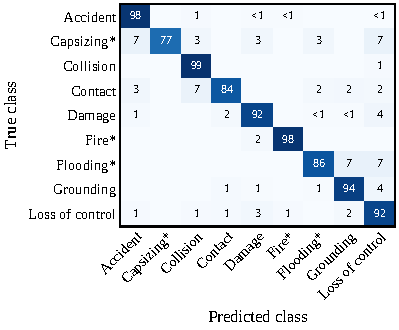
\includegraphics[width=\columnwidth]{figures/confusion_matrix.pdf}
\caption{Row-normalized confusion matrix of the best configuration, Att + wce + LLM augmentation, on the test set (two seeds summed). * marks safety-critical classes.}
\label{fig:cm}
\end{figure}

% --- Table V: top attention words per class --------------------------
\begin{table}[t]
\caption{The five words with the highest total attention weight per class, summed over correctly classified test reports (Att + wce, seed 1). Words shared by most classes (vessel, crew, crewmember, member, resulting, damage, suffered and experienced) are omitted.}
\label{tab:attention}
\centering
\footnotesize
\begin{tabular}{ll}
\toprule
Class & Top attention words \\
\midrule
Accident & fell, sustained, passenger, injury, fractured \\
Capsizing & capsized, hit, entered, boat, feathering \\
Collision & collided, pilot, manoeuvring, tanker, contact \\
Contact & contact, quayside, manoeuvring, struck, lock \\
Damage & \textbf{SOLAS, ladder, pilot, conform, regulations} \\
Fire & engine, caught, smoke, extinguish \\
Flooding & ingress, water, taking, started, motor \\
Grounding & grounded, ran, aground, yacht, whilst \\
Loss of Control & failure, engine, fouled, towed, propulsion \\
\bottomrule
\end{tabular}
\end{table}

Table~\ref{tab:attention} lists the words with the highest total attention weight for Att + wce. They are mostly the expected class indicators, e.g., \emph{capsized} for Capsizing, \emph{ingress} and \emph{water} for Flooding, and \emph{grounded} and \emph{aground} for Grounding. For Damage / Loss of Equipment, however, the top words are \emph{SOLAS}, \emph{ladder}, \emph{pilot}, \emph{conform} and \emph{regulations}. They point to a recurring subgroup of reports on pilot ladders that do not conform to SOLAS requirements, hidden within a broad class. This illustrates the value of attention for exploring reports, although attention weights show where the model looked, not why it decided \cite{jain2019attention,wiegreffe2019attention}.

Three observations suggest that the ceiling of about 0.91 macro-F1 comes from the single-label annotation rather than from model capacity: most dominant confusions are cause--consequence pairs or near-synonymous classes, related classes share top attention words (\emph{contact} appears among the top words of Collision), and a linear TF-IDF baseline comes within 0.03 macro-F1 of the best model.

\subsubsection{Limitations}
The results are based on two seeds and a single data split. The test set contains only 15 Capsizing reports, and none of the pairwise differences between configurations is statistically significant on it. Training was limited to five epochs, $\gamma$ and $\beta$ were not tuned, and only BERT-base was evaluated. The 1.5B-parameter LLM occasionally changed minor details, and its rewrites are more formal than the original reports. Future work should add seeds and data splits, evaluate domain-adapted encoders \cite{black2026domain}, and explore multi-label annotation that separates causes from consequences.

% =====================================================================
% 5. Conclusions
% =====================================================================
\section{Conclusions}\label{sec:conc}

This study developed a transformer-based framework for classifying marine incident reports and evaluated it on 5,762 public MAIB reports under a controlled protocol. The best configuration, BERT + BiLSTM + attention trained with weighted cross-entropy on LLM-augmented data, reached a macro-F1 of 0.915 and an accuracy of 93.5\%, against 0.885 and 91.4\% for a TF-IDF + SVM baseline. Most of this gain came from the weighted loss, while the BiLSTM and attention layers proposed in prior work did not improve on plain BERT beyond seed variation, nor did a larger BiLSTM, and LLM augmentation added little on top of the weighted loss. None of the differences between the BERT-based configurations is statistically significant on the 865-report test set. The residual errors are concentrated between cause and consequence classes, which suggests that better annotation schemes are a more promising direction than more complex architectures, and attention weights can help safety analysts find recurring subgroups such as non-compliant pilot ladders. Code and results are publicly available.\todo{add GitHub link once the repository is public}

% =====================================================================
% References (entries in refs.bib)
% =====================================================================
\bibliographystyle{IEEEtran}
\bibliography{refs}

\end{document}
